\documentclass{standalone}
\usepackage{mathpazo}
\usepackage[american voltages]{circuitikz}
\begin{document}
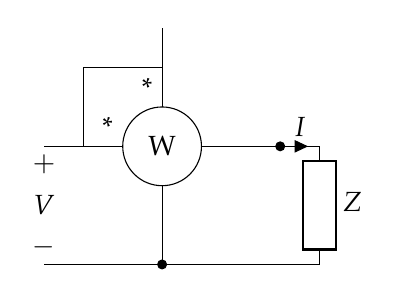
\begin{tikzpicture}
  \node at (0,0) {W};
  \draw (0,0) circle (0.5);
  \draw (0.5, 0) -- (1.5,0);
  \draw (-0.5, 0) node[above left] {*} -- (-1.5,0);
  \draw (0, 0.5) node[above left] {*} -- (0, 1.5);
  \draw (0, -0.5)  -- (0, -1.5);
  \draw (-1, 0) |- (0, 1);
  \draw (1.5, 0) to[short, *-, i=$I$] (2,0)
  to[european resistor, l = $Z$] (2, -1.5)
  to[short, -*] (0, -1.5)
  to[short, -] (-1.5, -1.5)
  (-1.5,0) to[open, v_=$V$] (-1.5,-1.5);
\end{tikzpicture}
\end{document}